% example.tex
\documentclass[dvisvgm]{standalone}

\usepackage[usenames,dvipsnames]{xcolor}
\usepackage{tikz}
\usetikzlibrary {arrows.meta,
                 positioning,
                 shapes.geometric}

\tikzset{
         square/.style={regular polygon, regular polygon sides=4},
         myarrow/.style={-Stealth, line width=0.25mm},
         doublearrow/.style={arrows={Stealth[length=1.5mm]-Stealth[length=1.5mm]}, line width=0.25mm},
}

\begin{document}
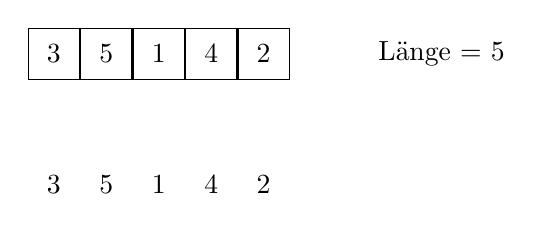
\begin{tikzpicture}
    % Grundmuster
    \node[draw, square] (a) {3}; 
    \node[draw, square, right=0cm of a] (b) {5};
    \node[draw, square, right=0cm of b] (c) {1};
    \node[draw, square, right=0cm of c] (d) {4};
    \node[draw, square, right=0cm of d] (e) {2};
    \node[right= of e] (e_text) {Länge = 5};

    % S1.1
    \node[square, below = of a] (a11) {3}; 
    \node[square, right=0cm of a11] (b11) {5};
    \node[square, right=0cm of b11] (c11) {1};
    \node[square, right=0cm of c11] (d11) {4};
    \node[square, right=0cm of d11] (e11) {2};
    


\end{tikzpicture}
\end{document}
